% Слияние путей исполнения по условию.
\subsection{Слияние путей исполнения по условию}

Универсальным способом векторизации программного кода, содержащего условия, является слияние всех путей исполнения под соответствующими предикатами.
Рассмотрим это действие на примере простого условия \texttt{cond}, по результату которого выполняется переход на один из блоков \texttt{block A} и \texttt{block B}.
Пусть известны вероятности переходов на эти блоки -- они равны $p$ и $1 - p$ соответственно.
Длины рассматриваемых блоков подберем таким образом, чтобы в сумме они давали единицу, а отношение их длин задавалось параметром $\alpha$.
Таким образом, длины блоков будут равны $\frac{\alpha}{\alpha + 1}$ и $\frac{1}{\alpha + 1}$ соответственно (см. рис.~\ref{fig:text_4_vec_mrg_under_cond_cond}).
При этом условимся считать, что длина блока и время его исполнения это по сути одно и то же (то есть, время исполнения блока исчисляется количеством содержащихся в нем операций).

\begin{figure}[ht]
	\centering
		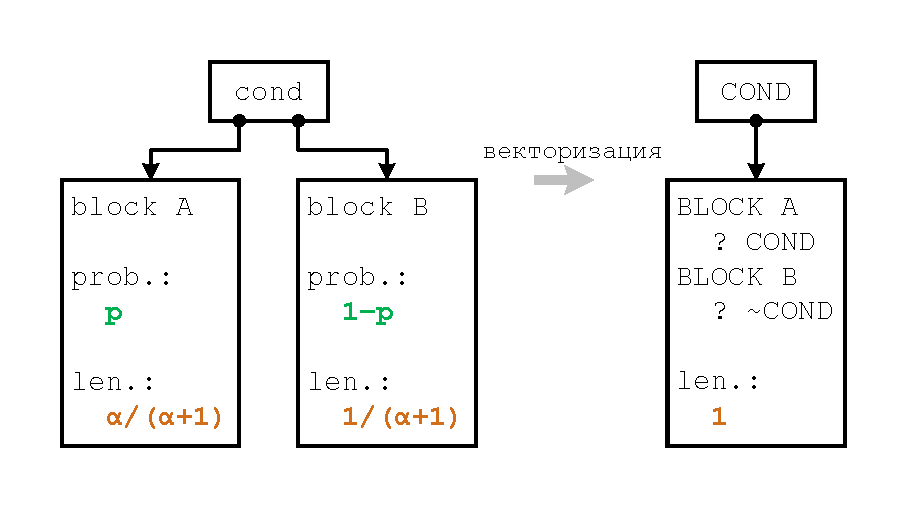
\includegraphics[width=0.8\textwidth]{./pics/text_4_vec_mrg_under_cond/cond.pdf}
	\caption{Схема векторизации участка программного кода, состоящего из одного условия и двух блоков, переход на которые осуществляется в соответствии с этим условием.}
	\label{fig:text_4_vec_mrg_under_cond_cond}
\end{figure}

Согласно представленной схеме программного контекста математическое ожидание времени исполнения рассматриваемых блоков в зависимости от условия, будет равно
\begin{equation}\label{eqn:text_4_vec_mrg_under_cond_t1}
	T_1 = \frac{p \alpha}{\alpha + 1} + \frac{1 - p}{\alpha + 1} = p\left(\frac{\alpha - 1}{\alpha + 1}\right) + \left(\frac{1}{\alpha + 1}\right).
\end{equation}

Время выполнения $w$ таких участков кода в невекторизованном виде будет равно $wT_1$.
При векторизации кода необходимо избавиться от операций перехода, вместо этого все операции блоков \texttt{block A} и \texttt{block B} должны быть поставлены под предикаты \texttt{cond} и \texttt{~cond} соответственно.
Далее выполняется объединение $w$ участков кода, при котором скалярные операции под предикатами \texttt{cond}, \texttt{\textasciitilde cond} заменяются на векторные аналоги, выполняющиеся с использованием векторных масок \texttt{COND}, \texttt{\textasciitilde COND}.
Так как длины блоков выбирались таким образом, чтобы в сумме они давали единицу, то время исполнения векторной версии кода в точности равно $T_w = 1$.
Таким образом, эффективность векторизации рассмотренного фрагмента кода совпадает со значением \eqref{eqn:text_4_vec_mrg_under_cond_t1} и равна
\begin{equation}\label{eqn:text_4_vec_mrg_under_cond_e}
	e = \frac{T_1}{T_w} = p\left(\frac{\alpha - 1}{\alpha + 1}\right) + \left(\frac{1}{\alpha + 1}\right).
\end{equation}

На рис.~\ref{fig:text_4_vec_under_cond_chart_e_merged} представлены графики зависимостей эффективности векторизации из \eqref{eqn:text_4_vec_mrg_under_cond_e} для разных значений параметра $\alpha$.

\begin{figure}[ht]
	\centering
		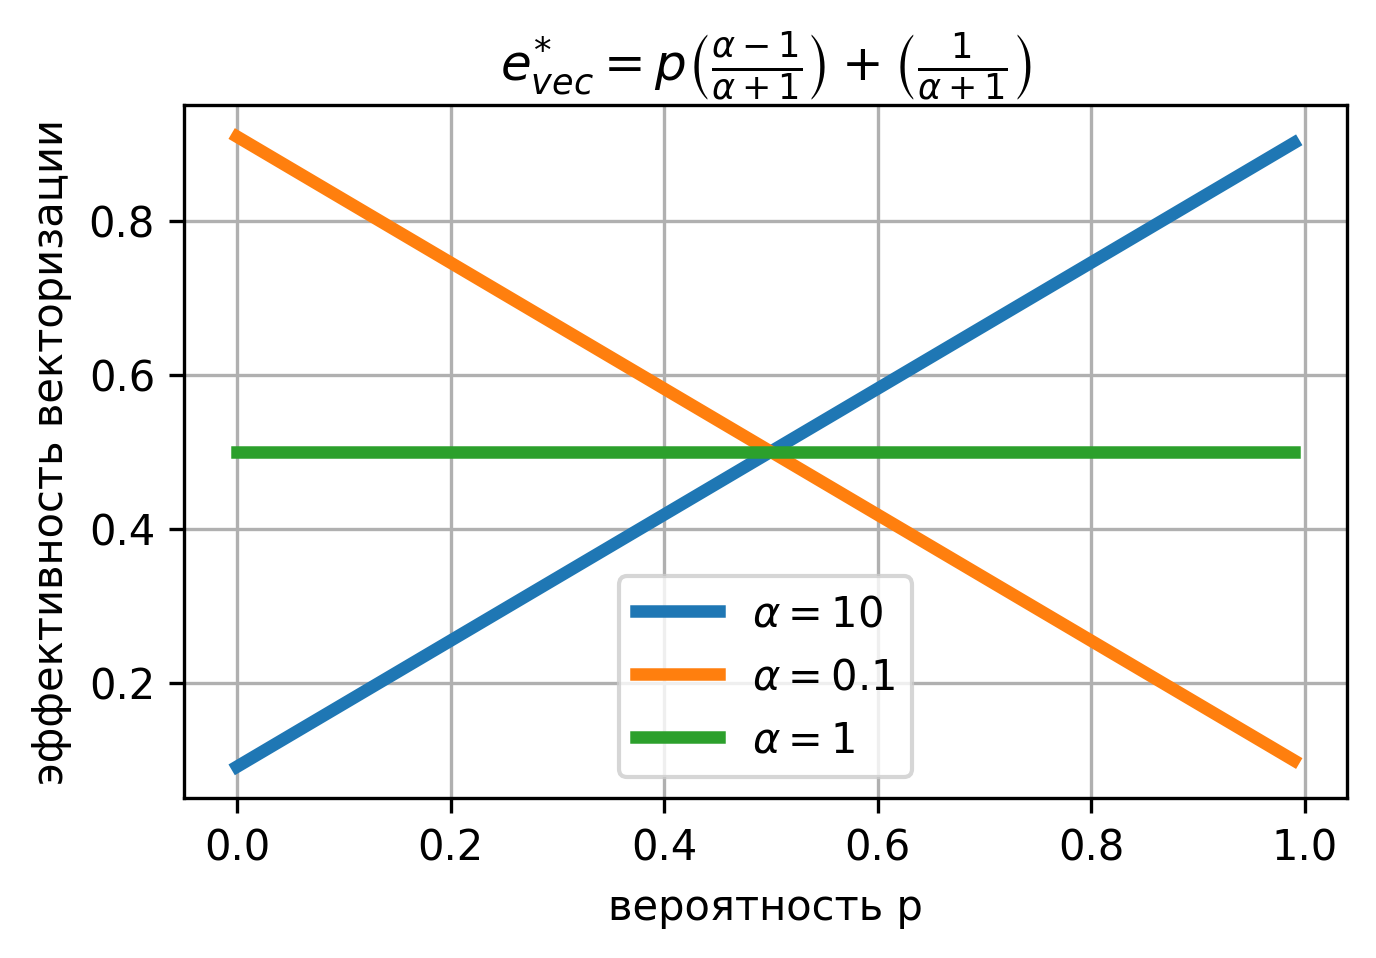
\includegraphics[width=0.6\textwidth]{./pics/text_4_vec_mrg_under_cond/chart_e_merged.png}
	\caption{Графики зависимостей эффективности векторизации от вероятности перехода на \texttt{block A} при значениях отношения длин блоков \texttt{block A} и \texttt{block B}, равных $10.0$, $0.1$, $1.0$ и при использовании простого слияния ветвей исполнения.}
	\label{fig:text_4_vec_under_cond_chart_e_merged}
\end{figure}

Из рис.~\ref{fig:text_4_vec_under_cond_chart_e_merged} видно, что при $\alpha = 1$ (то есть при одинаковых длинах блоков \texttt{block A} и \texttt{block B}) эффективность векторизации постоянна и равна $0.5$.
В тех же случаях, когда длины блоков отличаются, эффективность векторизации возрастает, если вероятность перехода на более длинный блок выше, чем на более короткий блок.
В любом случае, можно констатировать, что такой подход прямого слияния ветвей исполнения под соответствующими предикатами в единый линейный участок является крайне неэффективным.
При возрастании количества условий эффективность векторизации таким способом падает экспоненциально.
Это связано с появлением в программном коде большого количества векторных инструкций с практически пустыми масками.
Для повышения эффективности векторизации контекста с условиями требуется рассмотрение других подходов, позволяющих повысить плотность масок исполняемых векторных команд.
